\documentclass[a4paper,11pt]{article}

\usepackage[T1]{fontenc}
\usepackage[polish]{babel}
\usepackage[utf8]{inputenc}
\usepackage{lmodern}
\selectlanguage{polish}
\usepackage[top=2cm, bottom=2cm, left=3cm, right=3cm]{geometry}

\makeatletter
\newcommand{\linia}{\rule{\linewidth}{0.4mm}}
\renewcommand{\maketitle}{\begin{titlepage}
    \vspace*{2cm}
    \begin{center}\LARGE
    Politechnika Warszawska\\
    Wydział Elektryczny\\
    \end{center}
    \vspace{5cm}
    \noindent\linia
    \begin{center}
      \LARGE \textsc{\@title}
         \end{center}
     \linia
    \vspace{0.5cm}
    \begin{flushright}
    \begin{minipage}{5cm}
    \textit{Autorzy:}\\
    \normalsize \textsc{\@author} \par
    \end{minipage}
    \vspace{5cm}
     \end{flushright}
    \vspace*{\stretch{6}}
    \begin{center}
    \@date
    \end{center}
  \end{titlepage}%
}
\makeatother
\author{Grzegorz Kopyt\\
Daniel Sporysz}
\title{Specyfikacja Implementacyjna \\
"WireWorld"}

\usepackage{graphicx}
\begin{document}

\maketitle


\tableofcontents
\vspace{1cm}
\noindent\linia





\section{Diagram klas}


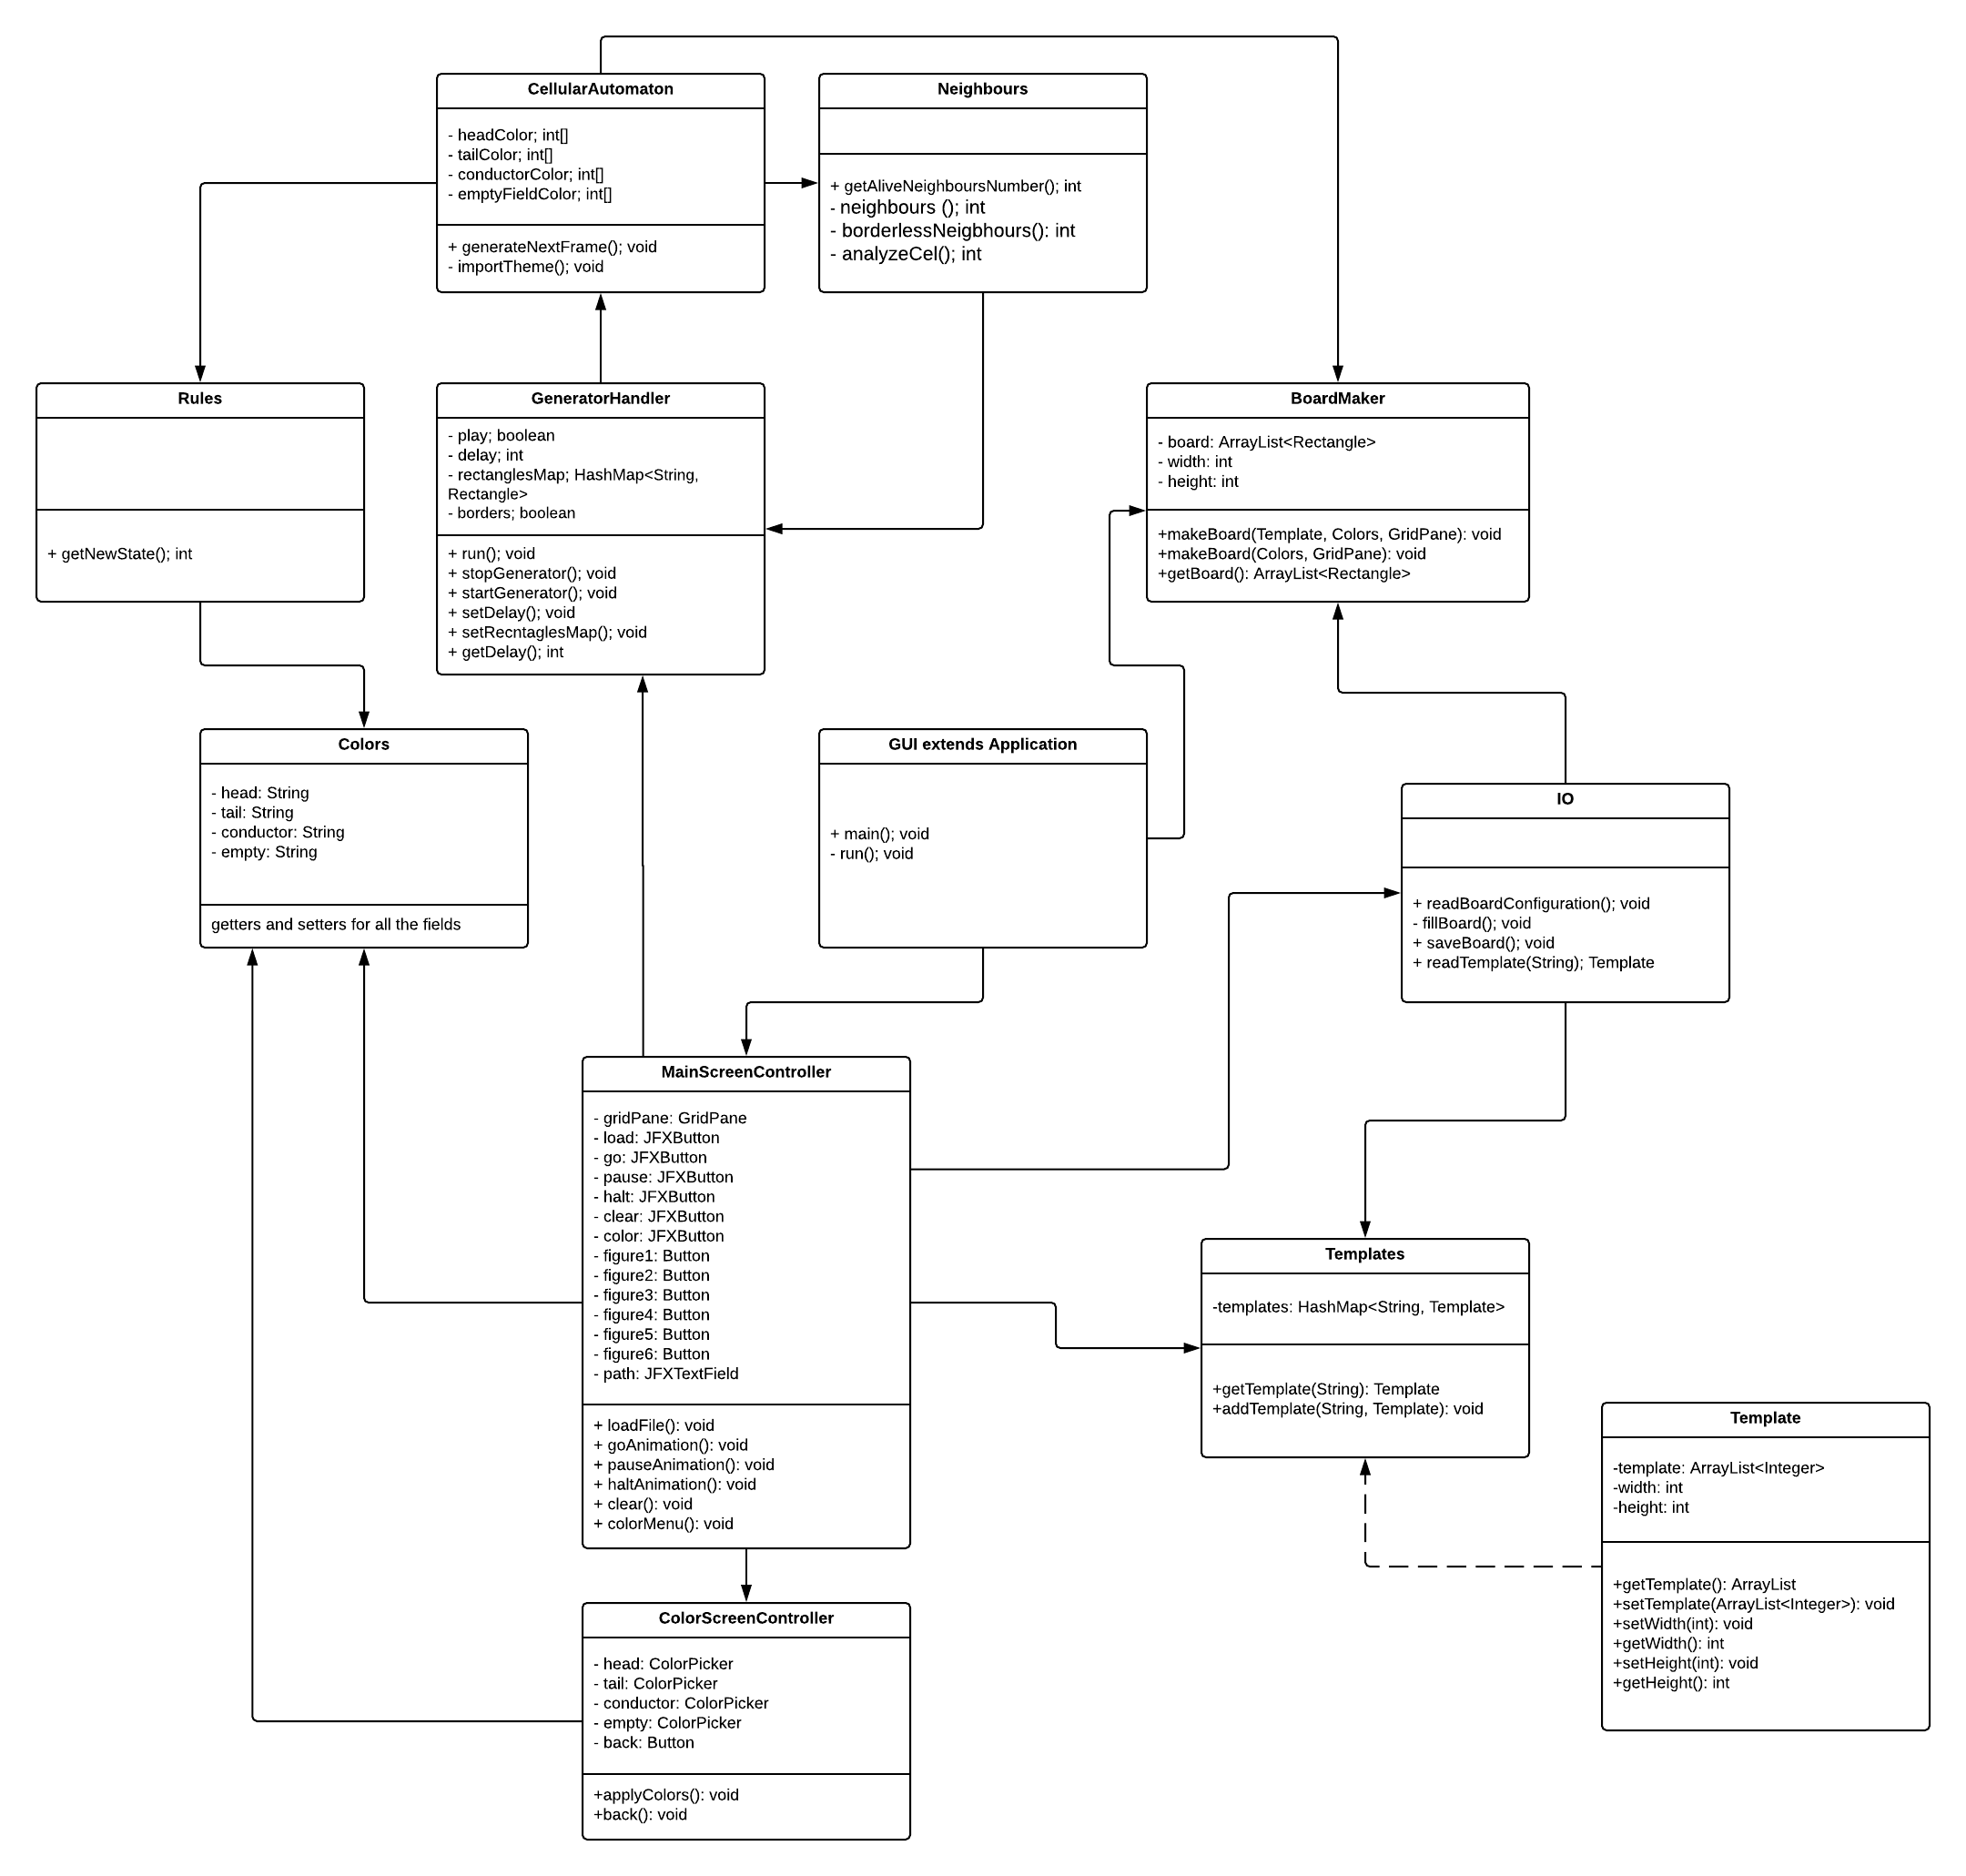
\includegraphics[width=\textwidth]{DiagramKlas}

\noindent\linia


\section{Diagram pakietów}
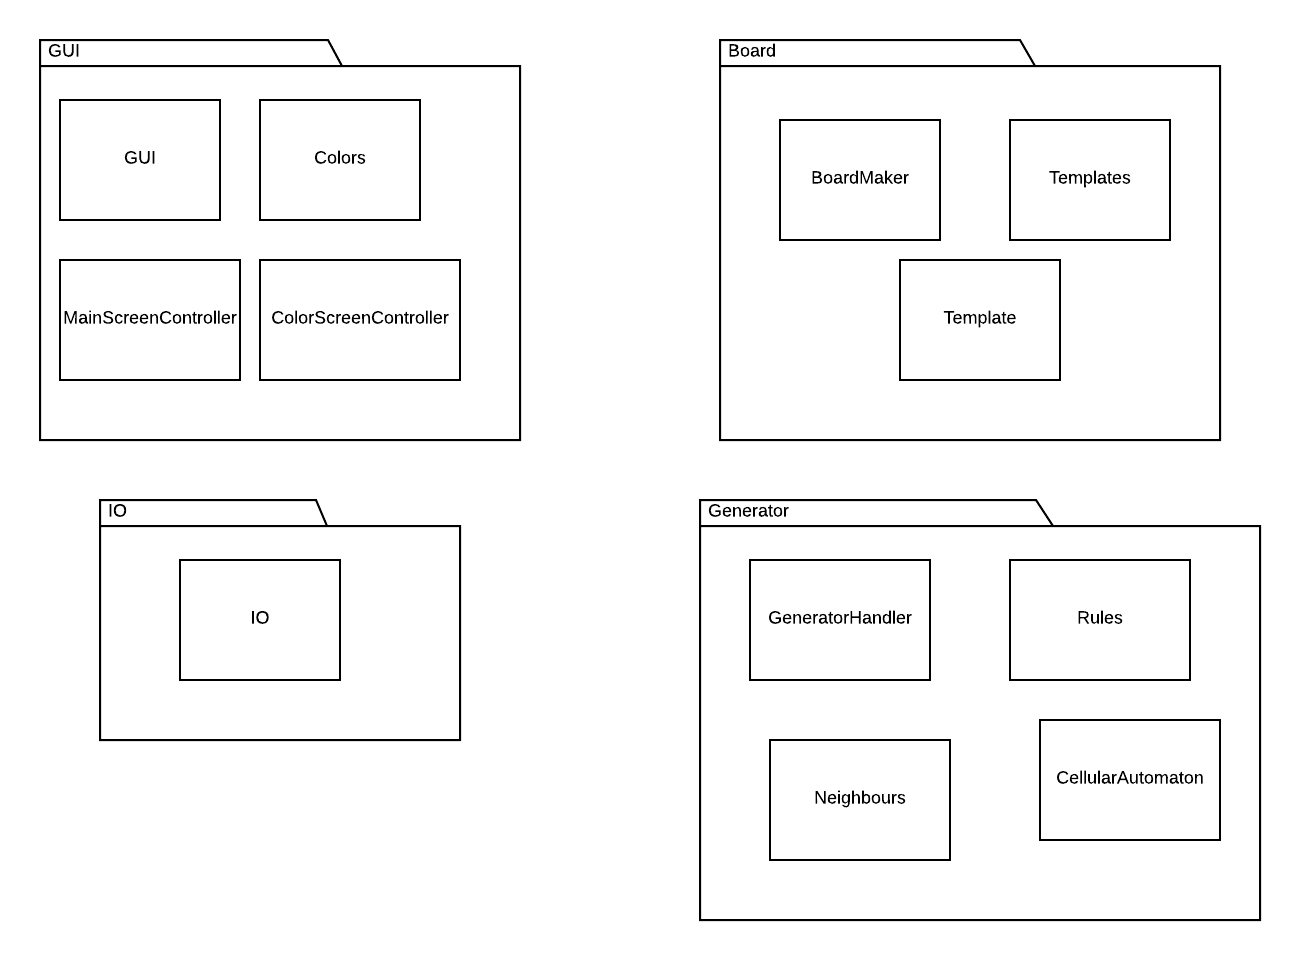
\includegraphics[width=\textwidth]{DiagramPakiet}







\noindent\linia
\section{Pakiet GUI}

Wykonany przy pomocy technologii javafx, zawiera dodatkową bibliotekę: jfoenix.

\subsection{Pliki .fxml:}
\begin{itemize}
\item MainScreen.fxml
\item ColorScreen.fxml
\end{itemize}

\subsection{GUI}
Rozszerza klasę Application z javafx.
\subsubsection{Pola}
brak
\subsubsection{Metody}
\begin{itemize}
\item \textbf{main}

Standardowo wywołuje metodę launch.
\item \textbf{start}

Wczytuje plik MainScreen.fxml, przygotowuje całą scenę i wyświetla ją w wymiarach (800, 600).
\end{itemize}


\subsection{MainScreenController}
Kontroler sceny MainScreen.fxml.
\subsubsection{Pola}
\begin{itemize}
\item GridPane \textit{gridPane}
\item JFXButton \textit{load}
\item JFXButton \textit{go}
\item JFXButton \textit{pause}
\item JFXButton \textit{halt}
\item JFXButton \textit{clear}
\item JFXButton \textit{color}
\item Button \textit{figure1}
\item Button \textit{figure2}
\item Button \textit{figure3}
\item Button \textit{figure4}
\item Button \textit{figure5}
\item Button \textit{figure6}
\item JFXTextField \textit{path}
\end{itemize}
\subsubsection{Metody}
\begin{itemize}
\item void \textbf{loadFile()}

Wywołuje metodę, która wczytuje plik tekstowy, którego ścieżkę podano w polu tekstowym.
\item void \textbf{goAnimation()}

Uruchamia animacje wywołując metodę z klasy Animation.
\item void \textbf{pauseAnimation()}

Pauzuje animacje metodą z klasy Animation.
\item void \textbf{haltAnimation()}

Powoduje powrót animacji do punktu początkowego.
\item void \textbf{clear()}

Zmienia kolor każdej komórki w tablicy na biały.
\item void \textbf{colorMenu()}

Wyświetla okno z pliku ColorMenu.fxml
\end{itemize}





\subsection{ColorScreenController}
Kontroler sceny ColorScreen.fxml.
\subsubsection{Pola}
\begin{itemize}
\item ColorPicker \textit{head}
\item ColorPicker \textit{tail}
\item ColorPicker \textit{conductor}
\item ColorPicker \textit{empty}

\end{itemize}
\subsubsection{Metody}
\begin{itemize}
\item void \textbf{back()}

Powoduje powrót do MainScreen.
\item void \textbf{applyColors()}

Pobiera z obiektów klasy ColorPicker informacje o kolorach i przekazuje je klasie Colors.

\end{itemize}
\noindent\linia




\subsection{Colors}
Kontroler sceny ColorScreen.fxml.
\subsubsection{Pola}
\begin{itemize}
\item String head
\item String tail
\item String conductor
\item String empty

\end{itemize}
\subsubsection{Metody}
\begin{itemize}
\item String \textbf{getHead()}
\item void \textbf{setHead()}
\item String \textbf{getTail()}
\item void \textbf{setTail()}
\item String \textbf{getConductor()}
\item void \textbf{setConductor()}
\item String \textbf{getEmpty()}
\item void \textbf{setEmpty()}
\subsubsection{Konstruktor}
Domyślne kolory to:
\begin{itemize}
\item head - żółty
\item tail - czerwony
\item conductor - czarny
\item empty - biały
\end{itemize}
\end{itemize}
\noindent\linia







\section{Pakiet IO}

\subsection{IO}

Klasa służy do odczytywania z oraz zapisu do polików graficznych konfiguracji pól na planszy.

\subsubsection{Pola}
\begin{itemize}
\item brak
\end{itemize}

\subsubsection{Metody}
\begin{itemize}
\item public void \textbf{readBoardConfiguration(String path, HashMap<String, Rectangle> map)}

Funkcja czyta plik graficzny o nazwie ,,path'', piksel po pikselu oraz zapisuje konfigurację do macierzy liczb całkowitych - reprezentujących stany komórek. 

Przy odczycie konieczna jest konwercja wartości z formatu RGB na jednocyfrowy znak stanu. Należy postępować według wzoru:
\begin{itemize}
\item RGB[ 230-255, 230-255, 230-255 ] -> 0
\item RGB[ 0-25, 0-25, 0-25 ] -> 1
\item RGB[ 230-250, 0-25, 0-25 ] -> 2
\item RGB[ 230-255, 230-255, 0-150 ] -> 3
\end{itemize}

Przedziały oznaczają tolerancję wariacji koloru.

Następnie wywołaj funkcje fillBoard.

\item private void \textbf{fillBoard(int[][] matrix, HashMap<String, Rectangle> map}

Metoda na podstawie otrzymanej macierzy liczb całkowitych, aktualizuje macierz ,,map'', zmieniając kolory obiektów zgodnie ze wzorem:
\begin{itemize}
\item 0 -> zmień kolor na biały
\item 1 -> czarny
\item 2 -> żółty
\item 3 -> czerwony
\end{itemize}

\item private void \textbf{saveBoard( String name, HashMap<String, Rectangle> map }

Funkcja zapisuje do pliku graficznego o nazwie ,,name'' konfigurację planszy.
\item public Template \textbf{readTemplate}

Funkcja odczytuje z pliku graficznego konfigurację wzoru, przy odczycie konwertując wartość koloru pikseli z formatu RGB na jednocyfrową liczbę całkowitą:

- 0 -> zmień kolor na biały

- 1 -> czarny

- 2 -> żółty

- 3 -> czerwony

A następnie zapisuje do obiektu Template i go zwraca. 
\end{itemize}

\noindent\linia

\section{Pakiet Board}

\subsection{BoardMaker}
Odpowiada za stworzenie tablicy obiektów klasy Rectangle (\textit{board}). Tablica ta będzie służyła jako obszar edytowany przez użytkownika, a także będzie na niej wyświetlana animacja.
\subsubsection{Pola}
\begin{itemize}
\item ArrayList<Rectangle> \textit{board}
\item int \textit{width}
\item int \textit{height}
\end{itemize}
\subsubsection{Metody}
\begin{itemize}
\item void \textbf{makeBoard(Template, Colors, GridPane)}

Metoda tworzy tablicę \textit{board} obiektów klasy Rectangle na podstawie wzoru podanego w Template o 30 kwadratach w rzędzie i 30 kwadratach w kolumnie.
Wymiary obiektów Rectangle wynoszą (20, 20).
Wszystkie obiekty dodane zostają do kolekcji \textit{board}.
Obiektom zostaje nadane ID jako kolejne liczby naturalne całkowite zaczynając od 1.
Kolor wypełnienia obiektów nadawany jest zgodnie z zawartością Colors, obramowanie - czarne.
Tablica tworzona jest poprzez dodanie obiektów do  GridPane.
Docelowy GridPane znajduje się w klasie MainScreenController.
\item void \textbf{makeBoard(Colors, GridPane)}

Metoda tworzy tablicę \textit{board} obiektów klasy Rectangle o 30 kwadratach w rzędzie i 30 kwadratach w kolumnie.
Wymiary obiektów Rectangle wynoszą (20, 20).
Wszystkie obiekty dodane zostają do kolekcji \textit{board}.
Obiektom zostaje nadane ID jako kolejne liczby naturalne całkowite zaczynając od 1.
Kolor wypełnienia obiektów nadawany jest zgodnie z zawartością Colors, obramowanie - czarne.
Tablica tworzona jest poprzez dodanie obiektów do  GridPane.
Docelowy GridPane znajduje się w klasie MainScreenController.

\item ArrayList<Rectangle> \textbf{getBoard()}
\end{itemize}



\subsection{Template}
Klasa reprezentująca wzór obiektu do wstawiania na tablice \textit{board}. Wzór przechowywany jest w tablicy \textit{template} jako ciąg liczb 0(pusty), 1(przewodnik), 2(ogon), 3(głowa). Przy tworzeniu wzorów należy uwzględnić to, że rozmiar tablicy wynosi 30 kwadratów na 30 kwadratów. 
\subsubsection{Pola}
\begin{itemize}
\item ArrayList<Integer> \textit{template}
\item int \textit{width}
\item int \textit{height}
\end{itemize}

\subsubsection{Metody}
\begin{itemize}
\item Template \textbf{getTemplate()}
\item void \textbf{setTemplate(ArrayList<Integer>)}
\item void \textbf{setWidth(int)}
\item int \textbf{getWidth()}
\item void \textbf{setHeight(int)}
\item int \textbf{getHeight()}
\end{itemize}


\subsection{Templates}
Przeznaczeniem klasy jest przechowywanie obiektów klasy template w kolekcji.
\subsubsection{Pola}
\begin{itemize}
\item HashMap<String, Template> \textit{templates}
\end{itemize}
\subsubsection{Metody}
\begin{itemize}
\item Template \textbf{getTemplate(String)}

Metoda otrzymawszy klucz klasy \textit{String} zwraca obiekt klasy Template z kolekcji \textit{templates}.
\item void \textbf{addTemplate(String, Template)}

Metoda dodaje do kolekcji \textit{templates} obiekt klasy Template i nadaje mu klucz podany jako zmienna klasy String.
\end{itemize}
\noindent\linia

\section{Pakiet Generation}



\subsection{GenerationsHandler}
Obiekt ten, jako rozszerzenie klasy ,,Thread'', zapewnia wątek na którym wykonywana będzie generacja kolejnych plansz. Klasa ma za zadanie obserwować zmiany jakie użytkownik wprowadza poprzez interfejs graficzny i po odpowiednim skonfigurowaniu, cyklicznie uruchamiać, bądź czekać na uruchomienie generatora.

\subsubsection{Pola}
\begin{itemize}
\item boolean \textit{play}
\item boolean \textit{borders}
\item int \textit{delay}
\item CellularAutomation \textit{generator}
\end{itemize}

\subsubsection{Metody}
\begin{itemize}
\item void  \textbf{run}

W nieskończonej pętli wywołuje metodę ,,generateNextFrame'', poprzednio sprawdzając wartość pola ,,play'', oznaczającego, czy generacja ma być wykonywana. Konstrukcja pętli umożliwia wstrzymywanie i wznawianie pracy generatora.
Kolejne uruchomienia generatora uruchamiane są w odstępach czasowych określonych w zmiennej ,,delay'' wyrażonej w milisekundach.
\item public void  \textbf{startGenerator}

Zmienia wartość pola ,,play'' na ,,true''.
\item public void  \textbf{stopGenerator}

Zmienia wartość pola ,,play'' na ,,false''.
\item public void  \textbf{setDelay(int value}

Przypisuje polu ,,delay'' wartość ,,value''.

\item int  \textbf{getDelay}

Zwraca wartość pola ,,delay''.

\end{itemize}

\subsection{CellularAutomaton}
Klasa pełni rolę generatora kolejnych plansz.

\subsubsection{Pola}
\begin{itemize}
\item int  \textit{boardWidth}
\item int  \textit{boardHight}
\item int[][] \textit{tmp}
\item HashMap<String, javafx.scene.shape.Rectangle> \textit{map}
\item int[]  \textit{headColor}
\item int[]  \textit{tailColor}
\item int[]  \textit{conductorColor}
\item int[]  \textit{emptyFieldColor}
\item Rules \textit{rules}
\item Neighbours \textit{neighbours}

\end{itemize}

\subsubsection{Metody}
\begin{itemize}
\item public void  \textbf{generateNextFrame( boolean borders )}

Na początku należy zaktualizować konfigurację kolorów za pomocą metody ,,importTheme''.

Następnie dla każdej komórki w mapie ,,map'', należy wywołać funkcje ,,getHeadNeighboursNumber'' oraz ,,getNewState'', a wynik zapisać pod odpowiedniej indeksem w tablicy ,,tmp''.

Po przeanalizowaniu całej planszy i zapisaniu nowych stanów do macierzy ,,tmp'', należy wyświetlić zmiany na ekranie, aktualizując kolory kwadratów w macierzy ,,map'', zgodnie z konfiguracja z ,,tmp''. Konwersja liczby całkowitej na kolor przebiega w następujący sposób:
\begin{itemize}
\item 0 -> emptyFieldColor
\item 1 -> conductorColor
\item 2 -> tailColor
\item 3 -> headColor
\end{itemize}

\end{itemize}

\subsection{Rules}
Klasa determinuje stan w który komórka przechodzi w następnej generacji, uwzględniając jej aktualny stan oraz stan komórek sąsiednich. 

\subsubsection{Pola}
\begin{itemize}
\item brak
\end{itemize}
\subsubsection{Metody}
\begin{itemize}
\item public int  \textbf{getNewState( int state, int headsNumber )}

Zależnie od otrzymanych argumentów funkcja zwraca:
\begin{itemize}
\item state = 0, zwróć 0
\item state = 3, zwróć 2
\item state = 2, zwróć 1
\item state = 1 i headsNumber != 1 != 2, zwróć 1
\item state = 1 i headNumber = 1 lub 2, zwróć 3

\end{itemize}

\end{itemize}

\subsection{Neighbours}
Obiekt zajmuje się analizowaniem stanów komórek. Jego zadaniem jest zwrócenie informacji o ilości komórek, które są ,,głowami'', dookoła konkretnej komórki. Sposób analizy można konfigurować.

\subsubsection{Pola}
\begin{itemize}
\item int  \textit{boardWidth}
\item int  \textit{boardHight}
\item HashMap<String, javafx.scene.shape.Rectangle> \textit{rectangleMap}
\end{itemize}
\subsubsection{Metody}
\begin{itemize}
\item public int  \textbf{getHeadNeighboursNumber( boolean borders, int x, int y )}

Funkcja pełni role przekaźnika. Jeśli zmienna ,,borders'' ma wartość true, wywołaj metodę ,,neighbours'', a w przeciwnym wypadku ,,borderlessNeigbhours''.

\item private int  \textbf{neighbours(int x, int y,)}

Funkcja sprawdza ile jest komórek w stanie HEAD(czerwony) dookoła komórki o pytanym indeksie. Indeksy spoza macierzy są ignorowane - pola poza macierzą mają stan różny od HEAD.
\item private int  \textbf{borderlessNeigbhours(int x, int y,)}

Funkcja sprawdza ile jest komórek w stanie HEAD(czerwony) dookoła komórki o pytanym indeksie. Indeksy spoza macierzy są zawijane, zamieniane na przeciwne.
\end{itemize}

\noindent\linia
\section{Przepływ Sterowania}

Przykładowe uruchomienie programu:
\begin{itemize}
\item start programu. 
\item start wątku generatora; GenerationsHandler.start()
\item przygotowanie okna interfejsu graficznego; GUI.
\item tworzenie tablicy komórek; BoardMaker.makeBoard()
\item określenie nazwy pliku i polecenie wczytania konfiguracji planszy z pliku 

- obsłużenie czynności przez MainScreenController
\item wywołanie funkcji czytającej z pliku; IO.readBoardConfiguration()
\item aktualizacja planszy; IO.fillBoard
\item użytkownik wciska przycisk start; MainScreenController
\item generatorHandler.startGenerator()
\item wątek GenerationsHandler rozpoczyna pracę i cyklicznie wywołuje CellularAutomation.generateNextFrame()
\item aktualizacja motywu kolorów; CellularAutomation.importTheme()
\item określenie liczby sąsiadów w stanie HEAD; Neighbours.getHeadNeighboursNumber()
\item określenie następnego stanu; Rules.getNewState()
\item Użytkownik wciska przycisk stop; MainScreenController
\item GeneratorHandler.stopGenerator()
\item wątek GenerationsHandler wstrzymuje pracę
\item użytkownik zleca zapis planszy do pliku graficznego; MainScreenController
\item zapis do pliku; IO.saveBoard()
\item użytkownik kończy pracę programu
\end{itemize}


\noindent\linia
\section{Testy klas i GUI}

\subsection{GUI}
\begin{description}

\item[Scenariusze] \hfill

\begin{enumerate}
\item Należy wpisać w pole tekstowe poprawną ścieżkę pliku (TestLoad.txt) i kliknąć w przycisk Load.
\item Należy wpisać w pole tekstowe niepoprawną ścieżkę pliku i kliknąć w przycisk Load.
\item Należy wpisać w pole 101 znaków.
\item Należy wpisać w pole tekstowe \textit{,,...!fte./tetat/assfs/////     "}.
\item Należy najechać myszką na planszę edycji.
\item Należy czterokrotnie kliknąć na dowolne pole planszy.
\item Należy przejechać po planszy ze wciśniętym lewym przyciskiem myszy.
\item Należy wyklikać na planszy taki wzór:

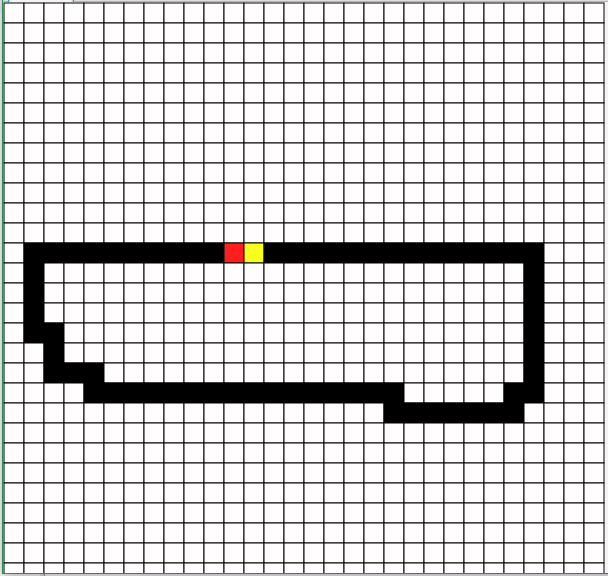
\includegraphics[width=\textwidth]{TestGUI1}
\item Po wykonaniu poprzedniego testu należy wcisnąć przycisk GO.
\item  Po wykonaniu poprzedniego testu należy wcisnąć przycisk Pause.
\item Po wykonaniu poprzedniego testu należy wcisnąć przycisk Halt!.
\item Należy kliknąć w przycisk Clear.
\item Kiedy na planszy są same białe komórki należy wcisnąć każdy z przycisków GO, Pause, Halt!
\item Dla każdego przycisku figure, należy: kliknąć na niego, następnie kliknąć na planszy w komórkę o współrzędnych (15,15) i komórkę (30,15)
\item Należy kliknąć w przycisk Color.
\item Należy ustawić plansze w sposób przedstawiony na obrazku poniżej.W oknie ColorMenu ustawić cztery różne kolory, następnie kliknąć przycisk back i kliknąć przycisk GO.

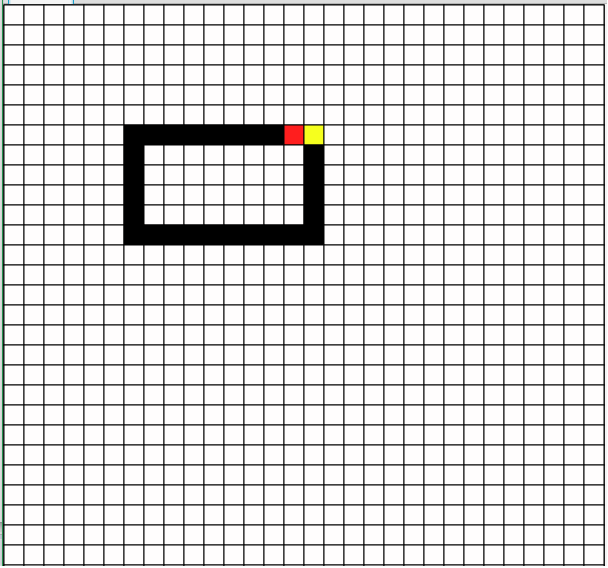
\includegraphics[width=\textwidth]{TestGUI2}
\end{enumerate}

\item[Kryteria oceny poprawnej pracy] \hfill
\begin{enumerate}
\item Jeśli na planszy pojawi się taki układ pól jak poniżej, test jest zaliczony.

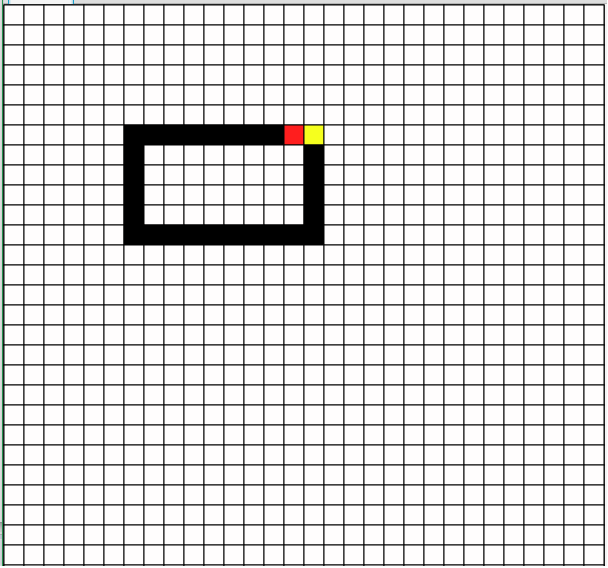
\includegraphics[width=\textwidth]{TestGUI2}
\item Program powinien wyświetlić w polu tekstowym czerwony komunikat ''Can't open the file.".
\item Program powinien wyświetlić w polu tekstowym czerwony komunikat ''Can't open the file.".
\item Program powinien pozwolić na wpisanie tylko 100 znaków.
\item Kolory nie powinny się zmienić.
\item Kolory powinny zmienić się cztery razy (czarny-->czerwony->żółty->biały).
\item Kolory powinny się zmienić o jeden.
\item Jeśli udało się to test jest zdany.
\item Kolory powinny się zmieniać zgodnie z zasadami wire world.
\item Animacja powinna się zatrzymać.
\item Animacja powinna wrócić do początkowego układu sprzed kliknięcia przycisku GO.
\item Wszystkie komórki powinny być białe.
\item Kolory na planszy nie powinny się zmieniać.
\item Elementy powinny zostać wstawione na plansze, z wyjątkiem przypadku, w którym zahaczają o krawędź ekranu.
\item Powinno pojawić się ColorMenu:

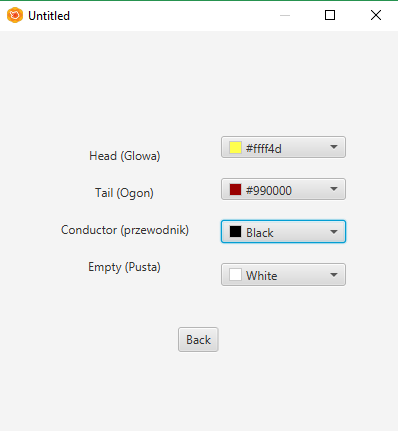
\includegraphics[width=\textwidth]{GUIWireWorld2}
\item Kolory na planszy powinny zostać zmienione zgodnie z ustawieniami, a animacja odbyć się zgodnie z zasadami wire world.
\end{enumerate}

\end{description}

\subsection{IO}
\subsubsection{IO}
\begin{description}

\item[Scenariusze] \hfill
\begin{enumerate}
\item Odczyt z pliku w formacie .png
\item Odczyt z pliku w formacie innym niż .png
\item Próba odczytu z pliku do którego brak praw odczytu
\item Zapis planszy do pliku .png
\item Próba zapisu planszy do pliku bez praw do zapisywania na dysku
\end{enumerate}

\item[Kryteria oceny poprawnej pracy] \hfill
\begin{enumerate}
\item Poprawny odczyt konfiguracji z pliku i aktualizacja komórek na ekranie
\item Obsłużenie wyjątków z brakiem praw do zapisu na dysk
\item Obsłużenie wyjątków z brakiem praw do czytania z dysku
\item Podanie ścieżki do pliku, który nie istnieje, bądź zawierającego niepoprawną konfigurację, skutkuje przerwaniem pracy i niezaktualizowaniem planszy.
\end{enumerate}

\end{description}

\subsection{Board}
\subsubsection{BoardMaker, Template}
\begin{description}

\item[Scenariusze] \hfill
\begin{enumerate}
\item Stworzyć obiekt Template jako wartości pól wymiarów podać (30, 30), a listę obiektów klasy Integer taką jak w pliku TestLoad.txt. Wypisać macierz na konsole.
\item Wywołać metode makeBoard w wariancie bez argumentu Template. Podając domyślny GridPane i obiekt Colors z domyślnymi kolorami.
\item Wywołać metode makeBoard w wariancie z argumentem Template takim jak w teście pierwszym. Podając domyślny GridPane i obiekt Colors z domyślnymi kolorami.

\end{enumerate}

\item[Kryteria oceny poprawnej pracy] \hfill
\begin{enumerate}
\item Jeśli macierz jest taka sam jak w pliku TestLoad.txt, test jest zdany.
\item W głównym menu interfejsu graficznego powinna pojawić się tablica białych kwadratów 30 na 30.
\item W głównym menu interfejsu graficznego powinna pojawić się taka tablica:

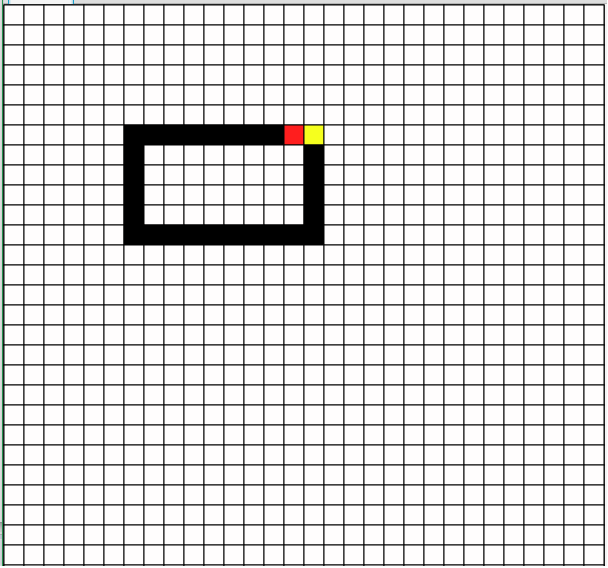
\includegraphics[width=\textwidth]{TestGUI2}
\end{enumerate}

\end{description}

\subsubsection{Templates}
\begin{description}

\item[Scenariusze] \hfill
\begin{enumerate}
\item Stworzyć puste obiekty Template, których pola x wypełnić kolejno wartościami 1, 2, 3. Dodać te obiekty do Tempaltes za pomocą metody \textit{addTempalte} nadając im  klucze 1, 2 ,3. Pobrać z Templates obiekty Template po kolejno 1, 2, 3 nadanych kluczach i wypisać wartości ich pól x na konsole.

\end{enumerate}

\item[Kryteria oceny poprawnej pracy] \hfill
\begin{enumerate}
\item  Na konsoli powinien pojawić się komunikat: ,,1 2 3"

\end{enumerate}

\end{description}

\subsection{Generation}
\subsubsection{GenerationsHandler}
\begin{description}

\item[Scenariusze] \hfill
\begin{enumerate}
\item pauzowanie i startowanie pracy generatora
\item zmiana parametru ,,delay''
\end{enumerate}

\item[Kryteria oceny poprawnej pracy] \hfill
\begin{enumerate}
\item Wątek reaguje na zmiany w konfiguracji programu

\end{enumerate}

\end{description}

\subsubsection{CellularAutomation}
\begin{description}

\item[Scenariusze] \hfill
\begin{enumerate}
\item analiza równobocznej planszy w dwóch trybach analizy
\item analiza nierównobocznej(poziomo)  planszy w dwóch trybach analizy
\item analiza nierównobocznej(pionowo) planszy w dwóch trybach analizy
\end{enumerate}

\item[Kryteria oceny poprawnej pracy] \hfill
\begin{enumerate}
\item Metoda przeanalizowała wszystkie pola HashMap'y map oraz za pomocą innych funkcji , wypełniła macierz ,,tmp''. Kończąc pracę funkcja poprawnie zaktualizowała stan obiektów w ,,map''.

\end{enumerate}

\end{description}

\subsubsection{Neighbours}
\begin{description}

\item[Scenariusze] \hfill
\begin{enumerate}
\item wywołanie funkcji dla poprawnych argumentów
\item wywołanie dla indeksów spoza macierzy
\item praca na tablicy zawierającej nierozpoznawane oznaczenia stanów

\end{enumerate}

\item[Kryteria oceny poprawnej pracy] \hfill
\begin{enumerate}
\item funkcja zwraca poprawną ilość sąsiadów w stanie HEAD, dookoła komórki o podanych indeksach
\item stany oznaczone nierozpoznawanym symbolami traktowane są jako pole w stanie pustym(0).

\end{enumerate}

\end{description}

\subsubsection{Rules}
\begin{description}

\item[Scenariusze] \hfill
\begin{enumerate}
\item wywołania z poprawnymi argumentami
\item wywołanie dla nieznanego stanu
\item wywołanie dla ujemnej liczby sąsiadów
\end{enumerate}

\item[Kryteria oceny poprawnej pracy] \hfill
\begin{enumerate}
\item funkcja zwraca wartości zgodne co do reguły określonej w opisie funkcji.
\item niepoprawny znak stanu lub liczba sąsiadów skutkuje zwróceniem 0.

\end{enumerate}

\end{description}


\end{document}



